% !TeX root = ../main.tex
% -*- coding: utf-8 -*-

\chapter{基于生成对抗网络特征提取的近边界数据研究}\label{3}

DNN分类器可以由其分类边界唯一的表示,本章将讨论DNN模型分类边界的具体表示方法,给出量化的分类边界距离定义,研究对抗性样本在源模型和派生模型上的可转移性以及生成近边界对抗性样本的方法和阐述DCGAN私有化近边界数据的详细过程。

\section{近边界对抗性样本}

DNN分类器的主要目标是对输入数据样本进行分类,因此,一个DNN分类器的特征通常由其决策模式和分类边界决定。分类器的分类边界是一个抽象的概念,我们无法直接描述它,但可以根据分类器的决策结果来间接的反应分类边界。下面给出分类器分类边界的定义:

\begin{myDef}
	\label{def:1}
	\pmb{分类边界}。给定一个数据样本$x$,如果数据样本$x$满足$g_i(x) = g_j(x)$,其中$i \neq j $并且$min(g_i(x), g_j(x)) > \mathop{max} \limits_{k \neq i, j}g_k(x)$,$g_k(x)$代表数据样本$x$被决策为类别$k$的概率,那么称数据样本$x$位于类别$i$和$j$的分类边界上。
\end{myDef}

注意,分类边界是DNN分类器的特征,是客观存在的,和我们是否能直接找到这样的数据点并不相关。因此,如何有效的获取分类边界或其附近的数据样本点,是本文方法要解决的问题之一。

模型窃取攻击是一种通过攻击目标模型并构建一个相似但不完全一样的模型来非法获取模型的技术。在这种攻击中,攻击者通常会对源模型进行修改,以便逃避模型所有者的检测。这些修改会导致源模型的分类边界发生变化,所以通常无法保证位源模型分类边界上的数据样本样本依旧位于可疑模型分类边界上。

对抗性样本是一类特殊的数据样本,它可以使得DNN模型输出异常的结果。虽然我们可以找到位于源模型分类边界上的对抗性样本,但是在经过修改的可疑模型中,因为分类边界的偏移,无法保证对抗性样本依然位于其分类边界上。因此,直接利用分类边界来作为模型指纹是脆弱的,因为模型修改会影响分类边界。

为了解决这个问题,与分类边界的思想类似,本文提出了一个鲁棒性更强的近边界数据概念。下面给出本文近边界数据的定义:

\begin{myDef}
	\label{def:2}
	\pmb{近边界数据}。给定一个数据样本$x$,一个阈值$\theta$,如果数据样本$x$满足$\vert g_i(x) - g_j(x) \vert \leq \theta$,其中$i \neq j $并且$min(g_i(x), g_j(x)) \geq \mathop{max} \limits_{k \neq i, j}g_k(x)$,$g_k(x)$代表数据样本$x$被决策为类别$k$的概率,则数据样本$x$被称为近边界数据。
\end{myDef}

近边界数据是指那些非常接近分类边界的数据样本,与位于分类边界上的数据样本类似,这些样本对模型的决策边界有重要的影响,因为它们能够揭示模型在边界附近的行为。由于近边界数据不要求样本完全位于分类边界上,因此即使模型分类边界发生偏移,仍然可以衡量数据近边界性。所以相对于直接使用分类边界来作为模型指纹,近边界数据在面对模型窃取攻击时有着更强的鲁棒性。

如图\ref{近边界数据示意图}所示,近边界数据位于DNN分类器的分类边界附近,其他数据的分布则离分类边界较远。判定是否为近边界数据由定义\ref{def:2}中的阈值$\theta$决定,当$\theta$较小时,近边界数据样本表现为更加靠近模型分类边界。

\begin{figure}[htbp]%%图,[htbp]是浮动格式
	\centering
	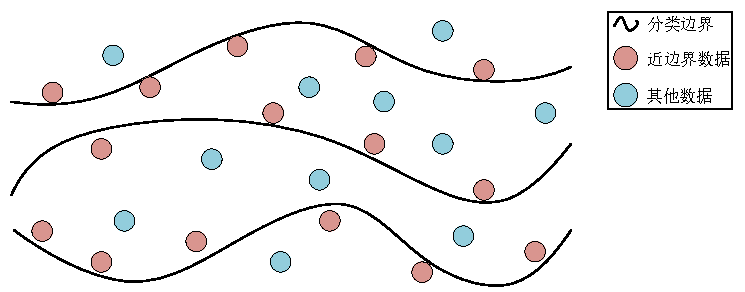
\includegraphics[width=12cm,height=8cm]{近边界数据示意图.pdf}
	\setlength{\abovecaptionskip}{5mm} %图片标题与图片距离
	\caption{近边界数据示意图}
	\label{近边界数据示意图}
	\end{figure}
	
相较于其他不相关的模型,对抗抗性样本可以更好的从源模型转移到其派生出的模型上。与对抗性样本类似,近边界数据也可以随着源模型转移,也就是说数据的近边界特性在派生模型上得到保留,详细的测试结果在\ref{5}\ref{5.2}中。在下一节中,我们将讨论如何生成所需的近边界对抗性样本。

\section{生成近边界对抗性样本}\label{3.2}

尽管近边界数据在模型的知识产权保护中表现出显著的效果,但是在实践中,获得一定规模的近边界数据样本仍然是一个具有挑战性的任务。这主要是由于自然的近边界数据在样本空间中的占比非常低,甚至可以被忽略不计,因此如何得到一定规模的近边界数据样本仍然是一个难题。

根据最近的一些研究\cite{cao2021ipguard},对抗性样本通常被用于确定分类器的分类边界。具体而言,对抗性样本有两个分类:原始分类和目标分类。其中,原始分类是指该样本不经过特殊处理的原始分类结果,目标分类是对原始样本添加微小噪声后的分类结果。对抗性样本是通过向原始数据添加小量扰动或干扰来生成的,这些扰动通常很难被人眼察觉,但却足以改变DNN模型的分类结果。

如图\ref{原始样本与对抗性样本对比}所示,对抗性样本对分类边界的跨越体现在,在视觉上,对抗性样本和原始样本几乎没有差别,但是分类结果却完全不同,在有目标攻击的情况下,甚至可以人为的指定目标分类。如在图\ref{原始样本与对抗性样本对比}中,原始样本的类别为石柱,对抗性样本却被分类器识别为高塔。

\begin{figure}[htbp]%%图,[htbp]是浮动格式
	\begin{minipage}[t]{0.49\linewidth}        %图片占用一行宽度的50%
		\hspace{2mm}
		\centering
		
\includegraphics[width=6cm,height=4.5cm]{对抗性样本原图.jpg}
		\centerline{(a)原始样本}
	\end{minipage}
	\begin{minipage}[t]{0.49\linewidth}        %图片占用一行宽度的50%
		\hspace{2mm}
		\centering
		
\includegraphics[width=6cm,height=4.5cm]{对抗性样本.jpg}
		\centerline{(b)对抗性样本}
	\end{minipage}
\setlength{\abovecaptionskip}{5mm} %图片标题与图片距离
\caption{原始样本与对抗性样本的对比}
\label{原始样本与对抗性样本对比}
\end {figure}

对抗性样本会对分类边界进行跨越,我们认为该特征可以帮助获得较多的近边界数据。具体来说,我们将生成大量的对抗性样本,并从中挑选合适的近边界数据。因此,本文测试了几种常见的生成对抗性样本的方法,以帮助我们更好的构建近边界数据。因为我们希望数据样本尽可能靠近分类边界,因此在测试过程中,不同方法的优劣取决于生成对抗性样本到分类边界距离的远近,距离近者更优。

为了更好的衡量数据样本到分类边界的距离,在定义\ref{def:2}的基础上,下面给出量化的分类边界距离定义:

\begin{myDef}
	\label{def:3}
	\pmb{分类边界距离}。给定一个数据样本$x$,它到分类边界的距离$distance = \vert g_i(x) - g_j(x) \vert$,其中$i \neq j $并且$min(g_i(x), g_j(x)) \geq \mathop{max} \limits_{k \neq i, j}g_k(x)$,$g_k(x)$代表数据样本$x$被决策为类别$k$的概率。
\end{myDef}

根据定义\ref{def:3},以分类边界距离为衡量标准,下面分别对几种常见的生成对抗性样本的方法进行介绍与测试。


\noindent\textbf{Fast \ Gradient \ Sign \ Method(FGSM):}FGSM \cite{goodfellow2014explaining}是最经典的生成对抗性样本的方法之一,它是一种基于梯度构建对抗性样本的方法,属于无目标的攻击方式。只需要对原始样本添加一次微小的扰动$\eta$,如式\ref{eq:3.1},\ref{eq:3.2}所示,即可生成样本$x$的对抗性样本$\tilde{x}$,十分高效。

\begin{equation}
	\label{eq:3.1}
	\eta = \epsilon \cdot sign(\bigtriangledown_xJ(\theta,x,y^*))
\end{equation}

\begin{equation}
	\label{eq:3.2}
	\tilde{x} = clip(x + \eta)
\end{equation}

\noindent 其中$sign$是符号函数,$x$表示原始样本,$y^*$表示$x$的真实类别,$\theta$表示模型权重参数,$J$表示分类器损失函数,$\bigtriangledown_x$表示对原始样本$x$求偏导,$clip$函数是将样本投射回可行数据域,比如图像样本的像素点范围应该在$[0,1]$以内,$\epsilon$用来控制变化幅度大小。

FGSM 生成对抗性样本的速度非常快,但其结果非常依赖$\epsilon$的选择,因此探索不同的$\epsilon$是使用该方法的重点。

\noindent\textbf{Iterative \ Gradient \ Sign \ Method(IGSM):}IGSM\cite{kurakin2018adversarial}是FGSM的进阶版本,如式\ref{eq:3.3},\ref{eq:3.4}所示,与FGSM只进行一次扰动叠加不同,IGSM采用迭代的形式构造对抗性样本,每次叠加一个小扰动。这个过程持续到成功生成对抗性样本或者达到迭代次数上限为止。

\begin{equation}
	\label{eq:3.3}
	\eta = \alpha \cdot sign(\bigtriangledown_xJ(\theta,x,y^*))
\end{equation}

\begin{equation}
	\label{eq:3.4}
	\tilde{x}_t = clip(\tilde{x}_{t - 1}  + clip_{\epsilon}(\eta))
\end{equation}

\noindent 其中$\alpha$是步长大小,$\tilde{x}_t$表示第$t$次迭代后的结果,$clip_{\epsilon}$是限定每次叠加的范围不超过$\epsilon$,其余参数含义与FGSM保持一致。

除此之外,我们还测试了FGSM的另一个进阶版本RFSGM\cite{tramer2017ensemble},RFSGM增加了扰动的多样性,可以更精细地生成对抗性样本。在实际结果中我们发现尽管FGSM生成对抗性样本速度非常快,但是对抗性样本距离分类边界的距离比较远。IGSM 和RFGSM 效果要比FGSM 好,但仍然没有达到我们的预期,生成的对抗性样本距离分类边界距离太远。在大量的测试中,我们发现CW能够生成大量位于分类边界附近的样本,具体的测试结果在\ref{5}\ref{5.2}中。

\noindent\textbf{Carlini \ and \ Wagner's \ methods(CW):}CW\cite{carlini2017towards}方法是一种有目标的攻击方式,同样是添加噪声到对抗性样本中,但其具有三种变体:CW-$L_0$,CW-$L_2$和CW-$L_{\infty}$,不同的变体使用不同的方法来衡量噪声的大小,其中CW-$L_2$在实验中生成对抗性样本的效果和生成效率相比其余两种变体较好,因此本文使用该方法作为生成对抗性样本的选择。具体而言,CW-$L_2$对于给定的初始样本,采用二分查找的方式来增大或减小式\ref{eq:3.7}中$c$,并且使用类似训练神经网络模型的方式来调整生成对抗性样本的其他参数。CW-$L_2$的损失函数和约束如式\ref{eq:3.5},\ref{eq:3.6},\ref{eq:3.7},\ref{eq:3.8}所示:

\begin{equation}
	\label{eq:3.5}
	Loss = Loss1 + Loss2 
\end{equation}

\begin{equation}
	\label{eq:3.6}
	Loss1 = D(x, x + \delta)
\end{equation}

\begin{equation}
	\label{eq:3.7}
	Loss2 = c \cdot f(x + \delta,target)
\end{equation}

\begin{equation}
	\label{eq:3.8}
	x + \delta \in [0,1]^m
\end{equation}

\noindent 其中$target$是生成对抗性样本的目标标签,$c$是惩罚因子,用于权衡$Loss2$的影响大小,算法通过二分查找来寻找合适的$c$。$Loss1$约束对抗性样本$x + \delta$和原始样本$x$尽可能相似,$Loss2$约束对抗性样本$x + \delta$的决策结果为目标标签,式\ref{eq:3.8}约束对抗性样本在正常的图像范围内。

根据定义\ref{def:3},数据样本$x$距离分类边界的距离是$distance = \vert g_i(x) - g_j(x) \vert$,本节的目标是生成的对抗性样本距离分类边界的距离尽可能近。我们在算法迭代过程中引入这一目标,以此改进算法迭代的过程,在使得生成对抗性样本更加靠近分类边界的同时,提高算法效率。具体而言,在迭代过程中,我们仅在$distance$变小时,更新距离参数和新生成的对抗性样本,并在$distance$小于等于预定的阈值$\theta$时,提前终止算法的迭代,具体的过程如算法\ref{alg:1}所示。

\begin{algorithm}[H] 
	\setstretch{1.3}
	\caption{改进的二分查找CW-$L_2$算法}
	\label{alg:1}
	\begin{algorithmic}[1]
		
		\Require 样本$x$;模型$M$;阈值$\theta$;二分次数$n$;迭代次数$iteration$;原始标签$r$;目标标签$t$
		\Ensure 近边界对抗性样本$x'$
		\State 参数初始化:$c\gets1$,$distance \gets 1$
		\For {$i=1,2,...,n$}
			\State $isSuccessAttack \gets false$
			\State $w \gets arctanh(x)$
			\State $w\_pert \gets zero\_like(w)$
			\For{$j=1,2,...,iteration$}
				\State $new\_img \gets tanh(w + w\_pert)$
				\State $new\_distance \gets \vert g_r(new\_img) - g_t(new\_img) \vert$
				\If{$new\_distance < distance$}
					\State $distance \gets new\_distance$
					\State $x' \gets new\_img$
					\State $isSuccessAttack \gets true$
				\EndIf
				\State 使用$Adam$更新$w\_pert$
			\EndFor
			\If{$isSuccessAttack == true$}
			\State 减小$c$
			\Else \State 增大$c$
			\EndIf 
			\If{$distance \leq \theta$} 
			\State $break$
			\EndIf
		\EndFor
		\State \textbf{return} $x'$
	\end{algorithmic}
\end{algorithm}

通过算法\ref{alg:1},我们已经可以生成大量位于分类边界附近的对抗性样本,即本文所需要的近边界数据。但是在这一阶段,我们只是在源模型的样本空间中挑选一部分数据作为初始样本添加微小噪声或扰动,针对性地生成了目标分类的对抗性样本。

在此阶段,源模型的训练和原始训练数据集均不受任何影响,防御者只需要针对性的生成对抗性样本即可。然而,近边界数据作为推断所有权的重要证据,直接生成对抗性样本也极易受到盗窃者的复制。因此,我们需要将生成的近边界数据私有化,防止盗窃者的模仿,具体操作将在下一节中给出。

\section{近边界数据私有化}\label{3.3}

因为现在大多数模型训练使用的数据都来源于公开的数据集,所以通过生成对抗性样本的方法构建近边界数据这一步骤也十分容易复现。因此我们需要从公开的训练数据中构建自己的私有化近边界数据,以防止模型所有者的近边界数据被轻易模仿,这是十分必要的,因为近边界数据是后续推断模型所有权的核心依据。

在本文中,我们希望可以通过训练一种模型学习上一节中生成的近边界对抗性样本的特征,并以此生成新的私有化近边界数据。这种新的数据从视觉上不一定和原始数据类似,但其原始的特征以及添加的噪声需要被学习,并根据提取到的特征生成的新样本对于源模型同样是近边界数据。因为本文用到的是图像样本,CNN可以很好的处理图像。因此,在本文中,我们设计了一种基于DCGAN\cite{radford2015unsupervised}的特征提取器,提取近边界数据的特征之后,使用生成器生成私有化的近边界数据。
%注意生成器以,$CW$-$L_2$生成的对抗性示例作为输入,并输出私有化后的近边界数据。

\begin{figure}[htbp]%%图,[htbp]是浮动格式
	\centering
	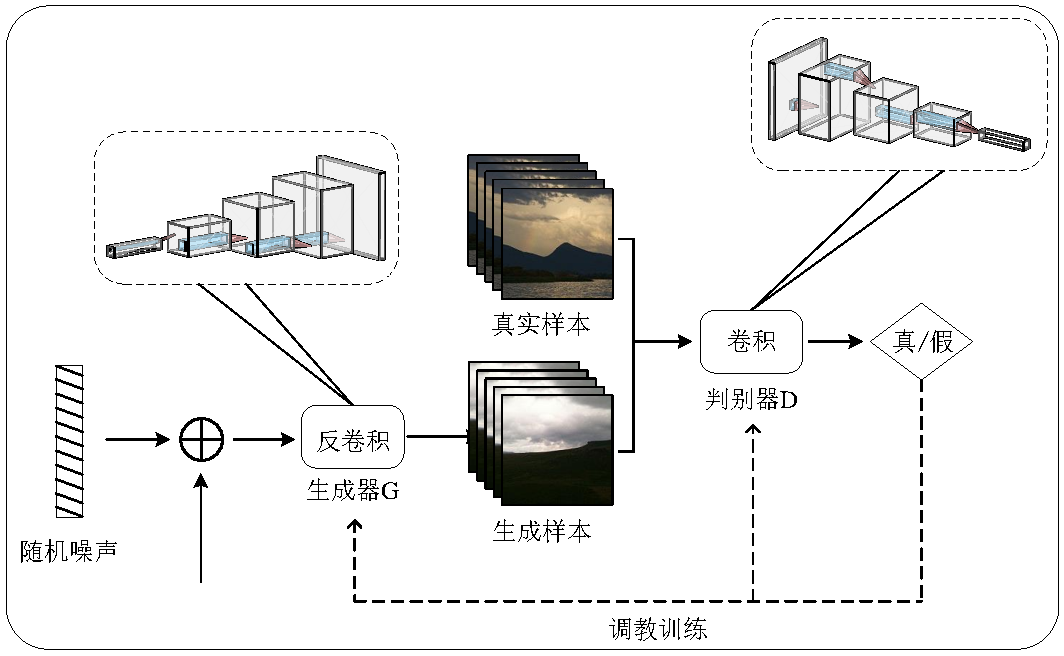
\includegraphics[width=14.5cm,height=9cm]{DCGAN网络结构图.pdf}
	%	\centerline{原始样本}
	\setlength{\abovecaptionskip}{5mm} %图片标题与图片距离
	\caption{DCGAN网络结构图}
	\label{DCGAN网络结构图}
\end {figure}

如图\ref{DCGAN网络结构图}所示,DCGAN的大体结构与训练方式和普通GAN类似,主要变化是DCGAN将原始的GAN与CNN结合到一起,生成器$G$和判定器$D$都用CNN架构替换了原始GAN的全连接网络。得益于CNN对图像的强大处理能力,DCGAN极大提升了网络训练稳定性和生成样本的质量。具体而言,DCGAN主要是从网络架构上改进了原始的GAN,主要改进如下:

\begin{enumerate}
	\renewcommand{\labelenumi}{\theenumi)}
	\item DCGAN的生成器和判别器均舍弃掉CNN的池化层,生成器使用反卷积层来还原图片,判别器保留CNN的整体架构,使用卷积层来提取图片特征。
	\item 在生成器和判别器中都使用Batch Normalization层,提升训练DCGAN模型稳定性的同时加速了训练。
	\item 生成器除最后一层使用Tanh激活函数外,其余层使用ReLU,判别器所有层均使用LeakyReLU,使模型可以更快的学习。
	\item 使用Adam优化器并调整了超参数,将学习率设置为0.0002,可以更好的学习到数据样本的特征。
\end{enumerate}

我们希望DCGAN能够学习到尽可能多的近边界数据特征,以便更好的生成近边界数据。训练过程中,尝试修改DCGAN判定器的目标函数,在保留梯度的情况下,将其与源模型的结果相连,即使用源模型和判别器共同判定是生成数据还是原始数据。这种方式得到的训练结果在同样的生成规模下略微优于原始DCGAN生成的数据。然而,考虑到两者的效率,实际情况下生成的结果并无较大区别,所以本文采用原始的训练方式。训练DCGAN的具体流程如算法\ref{alg:2}所示。

\begin{algorithm}[!h] 
	\setstretch{1.3}
	\caption{训练DCGAN模型}
	\label{alg:2}
	\begin{algorithmic}[1]
		
		\Require 近边界数据$\tilde{D}$;批处理大小$batchsize$;训练轮次$epoch$;损失函数$Loss$
		\Ensure 训练好的DCGAN模型
		\State 参数初始化:$learning \ rate \gets 0.0002$,$real\_label \gets 1$,$fake\_label \gets 0$
		\For{$i=1,2,...,epoch$}
		\State 随机噪声$z \gets 100$ 
		\State $x' \gets G(z)$
		\State $Loss1 \gets Loss(D(x), real\_label)$  \Comment $x$是近边界数据样本
		\State $Loss2 \gets Loss(D(x'), fake\_label)$
		\State $Loss_D \gets Loss1 + Loss2$
		\State $Loss_G \gets Loss(D(x'), real\_label)$ \Comment 生成器希望$D(x') $接近$real\_label$
		\State 使用$Adam$优化器更新生成器$G$,判别器$D$的网络参数
		\EndFor
	\end{algorithmic}
\end{algorithm}

通过算法\ref{alg:2},完成训练DCGAN模型后,DCGAN的生成器便可以作为近边界数据特征提取器。训练过程中,通过生成器和判定器的相互博弈,生成器生成图像的特征分布会愈来愈接近原始近边界样本。训练收敛时,生成器已经学习到近边界数据的特征。我们可以通过生成器生成私有的近边界数据,这样的数据仍然具备近边界性,且可疑对手无法轻易获得。

DCGAN对图像数据有着很强的特征提取能力,生成器能够很好的学习近边界数据特征,使用生成器构建的近边界数据位于目标分类边界附近。但是相比于原始近边界数据,由于随机因素,生成的数据样本近边界性会弱于原始近边界数据,我们仍然希望近边界数据最大程度上靠近目标分类边界。因为近边界数据与目标分类边界的距离越近,推断模型所有权成功的可能性就越大。此外,生成的私有近边界数据虽然只被模型所有者拥有,但对于一些功能易被泛化的模型,经过模型窃取攻击后,由于模型被修改,数据的近边界特性仍有可能被泛化。

因此,为了解决上述问题,本文提出使用近边界数据微调源模型的目标分类边界,使生成的私有近边界数据更加靠近DNN模型分类边界。如式\ref{eq:3.4}所示,$Loss_{FT}$是针对目标分类边界的损失函数。

\begin{equation}
	\label{eq:3.10}
	Loss_{FT} = \frac{1}{n} \sum^{n}_{i = 1} (g_t(x_i') - g_s(x_i'))^2
\end{equation}

\noindent 其中$n$是该目标分类边界的近边界数据的数量,$x_i'$是生成的近边界数据,$g_t(\cdot)$和$g_s(\cdot)$分别表示目标分类概率和源分类概率。

$Loss_{FT}$本质是希望近边界数据更靠近目标分类边界,但是为了尽可能减小对原始模型精度的影响,不能直接使用该损失函数对源模型进行微调。受DCGAN训练过程的启发,我们使用源模型的损失函数$Loss_{FM}$与$Loss_{FT}$两者交替训练微调源模型,并将学习率设置为0.0001,在保持源模型精度的同时,使生成的数据样本更加靠近目标分类边界。与DCGAN 的过程相似,这是一个博弈的过程,微调的具体流程如算法\ref{alg:3}所示。

\begin{algorithm}[H] 
	\setstretch{1.3}
	\caption{微调源模型}
	\label{alg:3}
	\begin{algorithmic}[1]
		
		\Require 原始数据集$D$;私有化近边界数据$D'$;批处理大小$batchsize$;训练轮次$epoch$;损失函数$Loss_{FT}$,$Loss_{FM}$;源模型$M$
		\Ensure 微调后的源模型$M'$
		\State 参数初始化:$learning \ rate \gets 0.0001$
		\For{$i=1,2,...,epoch$}                          
		\State $Loss1 \gets Loss_{FT}(g_t(x') , g_s(x'))$ \Comment $g_k(x')$:$x'$在第$k$类上的概率
		\State $Loss2 \gets Loss_{FM}(M(x), label)$ \Comment $label$指正常样本的原始标签
		\State 使用$Adam$优化器更新源模型$M$的网络参数
		\EndFor
	\end{algorithmic}
\end{algorithm}

\noindent 其中$x$指原始的数据样本,$x'$指DCGAN生成器生成的私有化近边界数据。

通过算法\ref{alg:3}微调目标分类边界使得私有近边界数据与源模型之间的联系更加紧密,这对后续能否成功推断模型所有权十分重要。在此算法中,我们只微调目标分类边界,且通过交替微调尽可能减少微调对源模型的影响。

\begin{table}[h]
	\centering
	\setlength{\arrayrulewidth}{0.5mm}
	\renewcommand\arraystretch{1.8}
	\caption{微调分类边界对模型的影响}
	\label{table:state}
	\begin{tabular*}{13cm}{@{\extracolsep{\fill}} l c c}
		
		\hline
		数据集        &    微调前准确率   &   微调后准确率            \\
		\hline
		CIFAR-10      &     0.886        &     0.873               \\
		
		Heritage      &     0.879        &     0.866               \\
		
		Intel\_image  &     0.854        &     0.846               \\
		\hline		
	\end{tabular*}
\end{table}

如表\ref{table:state}所示,正因为交替微调的设计和较小的学习率,源模型微调前后的精度差不超过3\%。因此,微调对于源模型的性能影响十分微小,甚至可以被忽略,但却有效提高了最后的所有权推断效果。更多微调目标分类边界对准确度的影响测试在\ref{5}\ref{5.4}中。


\section{本章小结}

本章主要描述了近边界数据的特性和生成近边界数据并将其私有化的过程。对抗性样本一般位于DNN模型分类边界上,并且可以很好的转移到其派生出的模型上。鉴于模型攻击一般会对源模型进行修改,本章提出了鲁棒性更强的近边界数据的概念,数据的近边界性也可以转移到其派生模型上,改变的是近边界数据到分类边界的距离。由于自然的近边界数据很少,本章对比了常见的生成对抗性样本的方法,在CW-$L_2$算法的基础上,引入了分类边界距离的概念来更快的生成近边界对抗性样本。考虑到敌手可能会产生近边界数据,我们设计了基于DCGAN的数据生成器,来私有化近边界数据,并在此基础上使用近边界数据微调源模型分类边界,提高所有权推断的置信度。
